% THIS IS SIGPROC-SP.TEX - VERSION 3.1
% WORKS WITH V3.2SP OF ACM_PROC_ARTICLE-SP.CLS
% APRIL 2009
%
% It is an example file showing how to use the 'acm_proc_article-sp.cls' V3.2SP
% LaTeX2e document class file for Conference Proceedings submissions.
% ----------------------------------------------------------------------------------------------------------------
% This .tex file (and associated .cls V3.2SP) *DOES NOT* produce:
%       1) The Permission Statement
%       2) The Conference (location) Info information
%       3) The Copyright Line with ACM data
%       4) Page numbering
% ---------------------------------------------------------------------------------------------------------------
% It is an example which *does* use the .bib file (from which the .bbl file
% is produced).
% REMEMBER HOWEVER: After having produced the .bbl file,
% and prior to final submission,
% you need to 'insert'  your .bbl file into your source .tex file so as to provide
% ONE 'self-contained' source file.
%
% Questions regarding SIGS should be sent to
% Adrienne Griscti ---> griscti@acm.org
%
% Questions/suggestions regarding the guidelines, .tex and .cls files, etc. to
% Gerald Murray ---> murray@hq.acm.org
%
% For tracking purposes - this is V3.1SP - APRIL 2009

\documentclass{acm_proc_article-sp}
\usepackage{multirow} 
\usepackage{array}
\usepackage{url}

\begin{document}

\title{MapReduce Resource Discovery and Monitoring Using Self-Organizing Multicast Trees}
%
% You need the command \numberofauthors to handle the 'placement
% and alignment' of the authors beneath the title.
%
% For aesthetic reasons, we recommend 'three authors at a time'
% i.e. three 'name/affiliation blocks' be placed beneath the title.
%
% NOTE: You are NOT restricted in how many 'rows' of
% "name/affiliations" may appear. We just ask that you restrict
% the number of 'columns' to three.
%
% Because of the available 'opening page real-estate'
% we ask you to refrain from putting more than six authors
% (two rows with three columns) beneath the article title.
% More than six makes the first-page appear very cluttered indeed.
%
% Use the \alignauthor commands to handle the names
% and affiliations for an 'aesthetic maximum' of six authors.
% Add names, affiliations, addresses for
% the seventh etc. author(s) as the argument for the
% \additionalauthors command.
% These 'additional authors' will be output/set for you
% without further effort on your part as the last section in
% the body of your article BEFORE References or any Appendices.

\numberofauthors{3} %  in this sample file, there are a *total*
% of EIGHT authors. SIX appear on the 'first-page' (for formatting
% reasons) and the remaining two appear in the \additionalauthors section.
%
\author{
% You can go ahead and credit any number of authors here,
% e.g. one 'row of three' or two rows (consisting of one row of three
% and a second row of one, two or three).
%
% The command \alignauthor (no curly braces needed) should
% precede each author name, affiliation/snail-mail address and
% e-mail address. Additionally, tag each line of
% affiliation/address with \affaddr, and tag the
% e-mail address with \email.
%
% 1st. author
\alignauthor
Kyungyong Lee\\
       \affaddr{ACIS Lab. Dept. of ECE}\\
       \affaddr{University of Florida}\\
       \email{klee@acis.ufl.edu}
% 2nd. author
\alignauthor
Tae Woong Choi\\
       \affaddr{ACIS Lab. Dept. of ECE}\\
       \affaddr{University of Florida}\\
       \email{twchoi@ufl.edu}
\alignauthor
Arijit Ganguly\\
       \affaddr{Amazon Web Services}\\
       \affaddr{Amazon.com}\\
       \email{arijit@amazon.com}
\and
\alignauthor
David I. Wolinsky\\
       \affaddr{ACIS Lab. Dept. of ECE}\\
       \affaddr{University of Florida}\\
       \email{davidiw@ufl.edu} 
\alignauthor
P. Oscar Boykin\\
       \affaddr{ACIS Lab. Dept. of ECE}\\
       \affaddr{University of Florida}\\
       \email{boykin@acis.ufl.edu}
\alignauthor
Renato Figueiredo\\
       \affaddr{ACIS Lab. Dept. of ECE}\\
       \affaddr{University of Florida}\\
       \email{renato@acis.ufl.edu}
}
\maketitle
\begin{abstract}
Resource monitoring and discovery are important processes for building a large computing system.
This paper presents a MapReduce-based resource discovering method, which runs on top of a structured Peer To Peer (P2P) network.
A self-organizing bounded-broadcast method allows our system to query the entire network efficiently with the latency cost of $O(log^2(N)))$, where $N$ is the number of nodes in a pool.
By using the concept of Map and Reduce functional programming model, our query system performs a matchmaking in each node with the local resource information,
and the matching result is summarized and aggregated in a distributed fashion at each node of the bounded-broadcast tree during the reduce phase.
Analysis and simulation results prove that our system is scalable with respect to the number of nodes. A performance comparison with SWORD, a DHT based resource query algorithm,
shows that our system imposes less update overhead when the number of resource attributes increases while providing more timely matching result.
MapReduce-based resource discovering system also supports new attribute addition without reconfiguring a previous state.
Our MapReduce-based query system is currently deployed on PlanetLab while built upon the Brunet P2P network. To our best knowledge, our system is the first demonstrated implementation of MapReduce-based resource monitoring system that runs on top of a P2P network.
\end{abstract}
\section{Introduction}
Desktop grids~\cite{bonic}~\cite{condor} using commodity computers connected over a local or wide-area network have been proven to be excellent platforms 
for high-throughput computing while providing sharing CPU power, storage  capacity, and applications.
These systems should be scalable, fault-tolerant, and secure in the presence of abnormal or malicious behavior of a user or churn. 
These systems must be able to distribute jobs evenly among nodes\footnote{We use terms \textit{node}, \textit{resource} and \textit{machine} interchangeably.} to achieve maximum utilization and alleviate hot stops. 
Middleware solutions such as Condor~\cite{condor} and Boinc~\cite{bonic} for managing distributed resources often rely on a centralized master server that has global view of available resources for optimal scheduling decisions. 
Worker nodes publish their resource information to the central master node that matches a job requirement against available resource information to determine the most suitable node that can execute a job. 
The master server approach often imposes significant administrative, uptime, and scalability issues, and the failure of the master can render all its managed resources unusable.  

Distributed Hash Table (DHT)~\cite{chord}~\cite{pastry} offers a decentralized information system that scales to a large number of nodes. 
It provides self-configuration in the presence of node failures, efficient object storage, and retrieval based on a key. 
Resource discovery often involves querying resources using attributes (CPU speed, disk space, RAM, and etc) by their desired values, often involving range queries on attributes. 
Thus, DHTs are often inadequate for these requirements. 
SWORD~\cite{sword} and Mercury~\cite{mercury} enhance the DHT to range and multi-attribute queries, but these systems cannot capture complex queries involving unstructured data, such as partial string matching or regular expression matching. 
To prevent hot spots where only a few nodes might end up storing bulk of information, they have to support a load balancing mechanism, which results in uneven node distribution.
Additionally, those systems require nodes to periodically publish their resource information, which can impose significant network overheads even when no jobs are being submitted to the system. 
Furthermore, the retrieved resource information might be stale due to characteristics of DHT entry update period. 
Finally, the usability of these systems in Network Address Translation (NAT) constrained environment is often unknown. 
In this paper we present a decentralized, self-organizing resource discovery system based on MapReduce that overcomes several of the above limitations of existing resource discovery systems. 
Our system stores resource information extracted by condor\_startd daemon~\cite{condor} locally at a node, 
and leverages a structured P2P network to create a multicast tree for efficient query dissemination and result aggregation over a large subset of nodes. 
A query to discover resources is propagated down the tree where each node performs a matchmaking using Condor Classified Advertisements (ClassAds)~\cite{classad} with requirements defined at Map function - the outcome of which is a rank that represents its ability to meet the job requirements; 
and each node propagates the query down to its child nodes in the multicast tree. 
Once leaf nodes have computed their Map functions, the results are communicated up the tree. 
Aggregation happens at each intermediate node by computing a Reduce function over the results obtained from its children. 

We present experiment results from a deployment of MapReduce based query system on PlanetLab~\cite{planetlab} with a structured P2P network, Brunet~\cite{brunet}. 
We compare the performance of our query system with SWORD~\cite{sword} analytically and through simulations.
Experiment results show that MapReduce-based query system completes querying 600 PlanetLab nodes within 15 seconds for 80\% of queries.
Our query system's characteristics and contributions are the following:
\begin{enumerate}
\setlength{\itemsep}{0pt}
\setlength{\parskip}{0pt}
\item No resource information update traffic: Each query is resolved using local up-to-date resource information.
\item Bounded-broadcast trees provide an efficient way to disseminate queries and reduce response message size.
\item By using well-known Map and Reduce functional programming model, programmers can implement parallel resource monitoring jobs in a distributed system easily.
\end{enumerate}
Based on our knowledge and survey, MapReduce-based query system is the first demonstrated implementation of MapReduce application deployed on a structured P2P network.
The rest of this paper is organized as follows. 
Section 2 discusses the MapReduce-based query system architecture. 
Section 3 evaluates the system and compares the performance with that of SWORD by simulation and analysis. Section 4 discusses related works.
Section 5 summarizes and concludes this paper.

\section{System architecture}
In this section, we describe the overall architecture of the MapReduce-based query system and the bounded-broadcast method. 
We will also discuss how we use Map and Reduce functions to handle query and response processing.
\subsection{Bounded-broadcast}
\begin{figure}[t]

\centering
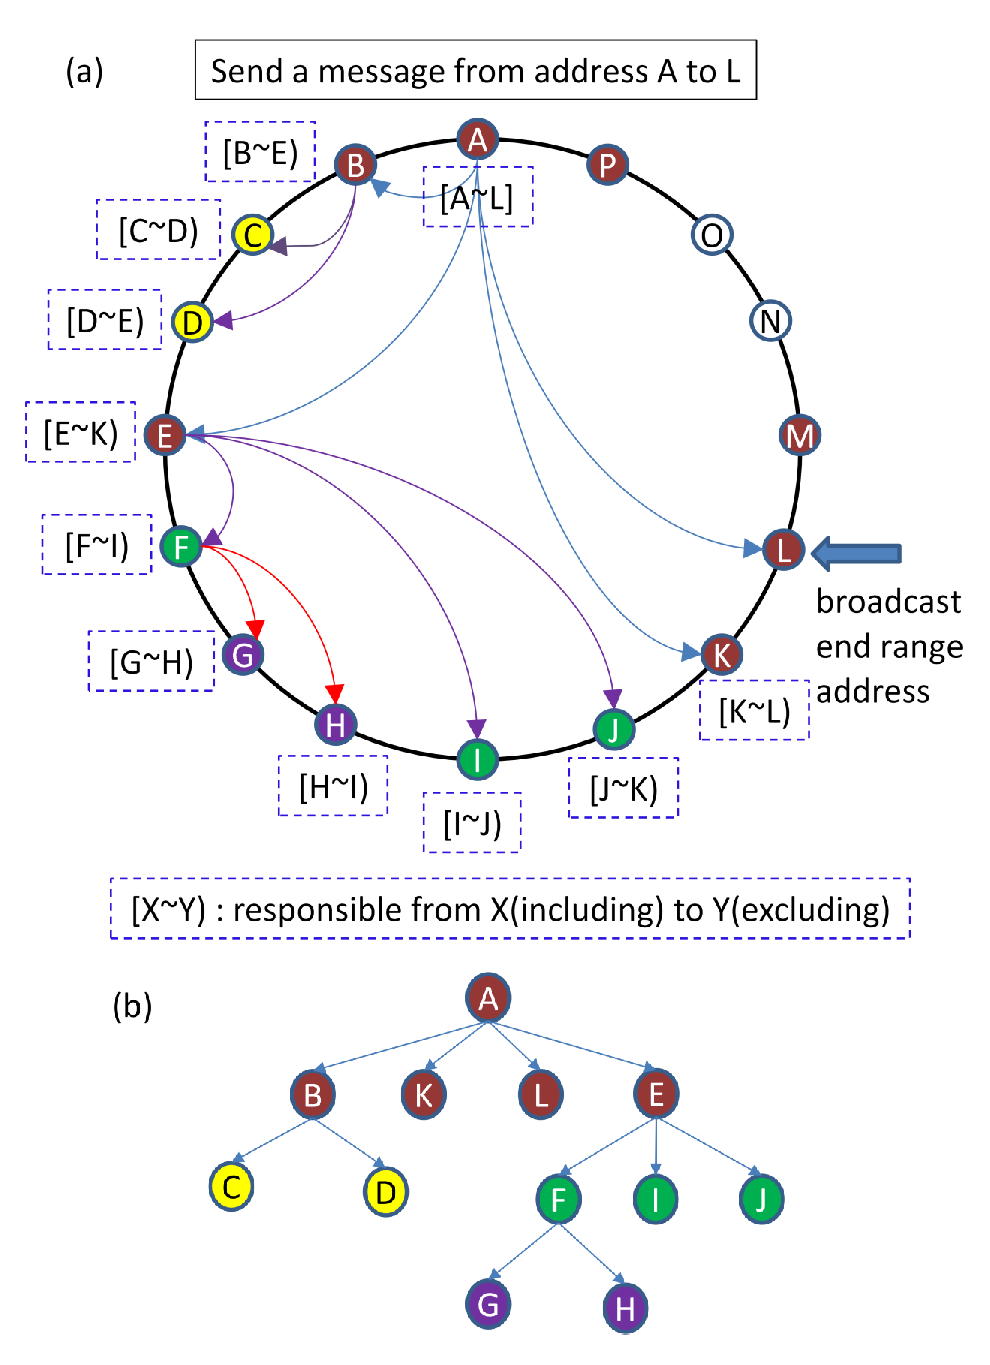
\epsfig{file=bb_tree.eps, width=3.4in}
\caption{Bounded-broadcast message propagation- (a) Node A broadcasts a message from node A to L. Node A first sends the message to its neighboring nodes, B, E, K, and L after setting broadcast region appropriately.
The message recipient node sends the message to its neighbors inside its broadcast region recursively. (b) Generated bounded-broadcast tree after disseminating the message.
\label{figure:bb}
}
\end{figure}
MapReduce-based resource discovery system uses bounded-broadcast~\cite{deetoo} to propagate queries. It spreads a message over a sub-region of a P2P network by leveraging a structured P2P system to self-organize a multicast tree. 
Bounded-broadcast is currently implemented on top of Brunet~\cite{brunet}, which implements a 1-d Kleinberg's small-world network~\cite{small_world_network}.
Each node maintains two types of connections: (1) constant number of near connections to its left and right neighbors on the P2P ring, and (2) about $0.5*log(N)$, where $N$ is the number of nodes, far connections to random nodes on the P2P ring; such that a routing cost is $O(log^2(n))$.

A node is allocated a sub-region of the P2P ring over which to disseminate a message. The node then redistributes the message to its neighbor nodes inside its allocated sub-region while allocating new sub-regions to the neighbor nodes. This process continues until the message is disseminated over the entire sub-region. 
For example, to broadcast a message over the sub-region [A,L] in Figure~\ref{figure:bb}, a message initiator issues a broadcast command to node A with sub-region information, [A,L]. 
Node A recognizes node B, P, E, K, L, and M as neighbors.
The node A then broadcast messages to its neighbors, by specifying broadcast range as [B~E), [E~K), [K~L), [L] to node B, E, K, and L, respectively.
After receiving the message, node B, E, K, and L broadcast the message only to their neighboring nodes inside the specified sub-region recursively. 
After disseminating the broadcast message until the leaf node, a graph like Figure 1 (b) is formed.

If a message initiating node does not lie within the bounded-broadcast domain (sub-region of the P2P ring), the message is first routed to a center node inside the bounded-broadcast region by using greedy routing.
The bounded-broadcast method is responsible for distributing arbitrary queries to nodes in a P2P pool and dealing with lagging nodes whose response time takes longer than the others. 
The latency cost of bounded-broadcast is $O(\log^2(N))$~\cite{deetoo}, which is larger than a DHT system $O(\log(N))$~\cite{chord}, but smaller than a naive flooding based broadcast method $O(N)$.

\subsection{MapReduce}
Map and reduce functions are popular paradigms in functional programming languages (Ruby, Python, LISP). 
A map function transforms each element ($x_i$) in a collection ({$x_1, x_2... x_n$}) into a different key element ($y_i$), thus creating a collection of intermediate elements ({$y_1, y_2... y_n$}).
A reduce function computes an aggregation ($z$) over this collection. 
Based on the concept of map and reduce functional programming model, software frameworks (Hadoop~\cite{hadoop} and Google~\cite{google_mapreduce}) have been developed to parallelize computations on large datasets efficiently. 
Map function usually works on (Key/Value) pairs to create intermediate (Key/Value) results. 
Reduce functions work on intermediate (Key/Value) results while aggregating intermediate values associated with the same intermediate keys. 
The framework distributes map and reduce tasks among nodes in a cluster to enable parallel processing, while users only have to specify the appropriate map and reduce functions associated with their computation without having to worry about details of distributed parallel job execution.  

In our MapReduce-based query system, we define the Map function as checking requirement matching and calculating a rank value. The Reduce function is defined as 
aggregating and ordering the Map result based on the matching result and rank value. These are presented in detail next.

\subsection{MapReduce Query System Architecture}
MapReduce-based query system is divided into 5 modules. They are P2P network module, MapReduce core, Map and Reduce function, local resource information monitor, and matchmaking module.
\subsubsection{P2P Network Module}
The P2P network module is responsible for handling new node join and departure, connection management with neighboring nodes, and routing messages. 
The current version of MapReduce query system is developed on top of Brunet~\cite{brunet}.
However, our system can be deployed on the other P2P platforms, such as Chord~\cite{chord}, CAN~\cite{can}, or Pastry~\cite{pastry}.

\subsubsection{MapReduce Core Module}
The MapReduce core module is responsible for distributing Map and Reduce functions using bounded-broadcast. 
When a user initiates a MapReduce task, the request is conveyed to the MapReduce core module through the underlying P2P network's Remote Procedure Call (RPC) module. 
The MapReduce core module checks the Map argument, Reduce argument, and broadcast region argument. 
The Map and Reduce argument will be passed to the Map and Reduce function, respectively. 
The broadcast region argument describes a bounded-broadcast region that the node is responsible for. 
The MapReduce core module disseminates the task to nodes which reside under its responsible region after manipulating broadcast region argument appropriately.
\subsubsection{Map and Reduce Function Module}
A user has to define own Map and Reduce functions associated with his needs. 
After a node processes the Map task, the node returns the Map result to the Reduce function of itself.
The Reduce function aggregates its own Map result and child nodes' Reduce results. 
After completing the Reduce function, the node returns the Reduce result to the parent node's reduce function.
For the resource discovering purpose, Map and Reduce functions are defined as follows:\\*\\*
\textbf{Map function}: A resource requirement and a rank criteria are delivered as a Map argument .
The following example illustrates a Map argument based on Conodr ClassAd.\footnote{We modified ClassAd syntax in this example for readability.}\\*\\*
\textit{Requirement} = (Memory>2048) \&\& (KeyboardIdle>300) \&\& (SoftwareInstalled.Contains("Matlab"))\ \ \ \ \ \ \ \ \ \ \ \ \ \ \ \ \ \ \ \ \ \ \ (1)\\*\\*
\textit{Rank} = (Memory) + (KeyboardIdle*10) \ \ \ \ \ \ \ \ \ \ \ \ \ \ \ \ \ \ \ \ \ \ \ \ (2)\\*\\*
Statement (1) describes the resource requirement. It means that the target resource's memory has to be bigger than 2GB and the keyboard idle time is more than 300 seconds.
The target machine also has to contain string \textit{Matlab} in a SoftwareInstalled attribute.
When a node receives a resource matching request, it first checks whether it satisfies the requirement or not. If it does, it calculates the rank value whose purpose is to order candidate nodes.
As users' demands change, it is highly likely that new attributes are added to the original resource attribute set. 
In this situation, using ClassAd allows users to add new attributes to the original resource attribute set easily.
Though a DHT-based query system usually supports adding new attributes to the original attribute set, it may result in performance degradation or rearranging whole DHT entries for new attributes.
Statement (2) shows the rank criteria. Every node which satisfies the requirement calculates its rank value using the given rank criteria, and this value is used to select optimal candidates.
As we can see from this example, a user can easily specify its requirement and rank value arbitrary.
For a matchmaking purpose, we use Condor ClassAd~\cite{classad} to exploit its regular expression and arbitrary matching support.
Using Condor ClassAd allows us ordering requirement satisfying nodes with more flexibility than related approaches such as~\cite{can_query}, which supports only a static ordering method (i.e., based on an average queue size and CPU speed).

\textbf{Reduce function}: In the Reduce function, the number of desired nodes and a rank ordering method are delivered as an argument.
Assuming that a node sends MapReduce tasks to $n$ nodes using bounded-broadcast, \begin{math}n\end{math} reduce results will be returned from child nodes, 
and one Map result will be returned from itself. The Reduce function will summarize those results based on the number of desired nodes, an ordering method, and rank values. 
The number of desired nodes specifies how many nodes the user wants to find in the pool, and an ordering method specifies a rank value alignment method. 
If the number of desired nodes is $k$, and the ordering method is \textit{ascending}, the rank value is aligned in the ascending order, and top \textit{k} rank value nodes are returned from the Reduce task.
As with Map, Reduce is processed at each node in a tree, and results are propagated back through the tree.
\begin{figure}
\centering
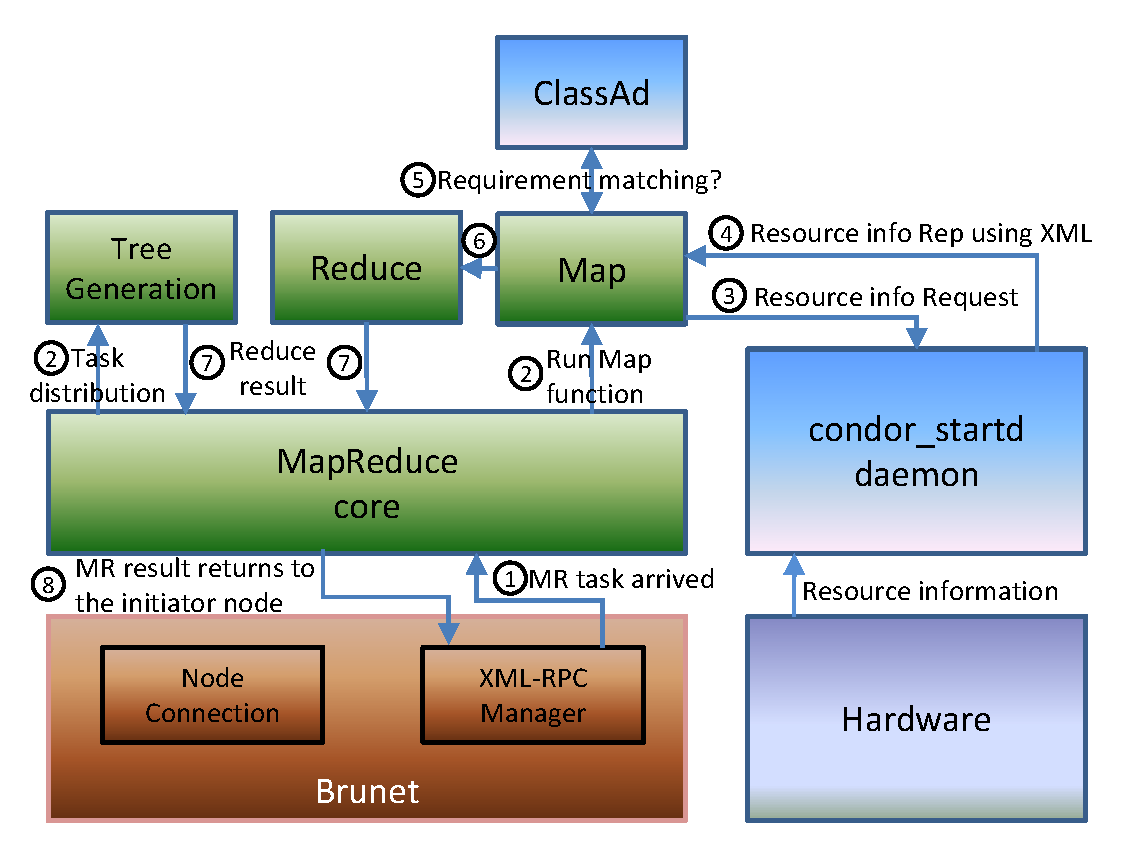
\epsfig{file=structure.eps, width=3.5in}
\caption{\label{fig:mr_arch}MapReduce query system architecture}
\end{figure}
\subsubsection{Local Resource Information Monitor Module}
There are several ways to gather resource information. The naive way would be using \textit{/proc} file system on a Linux machine. 
By using the \textit{proc} file system, we can get a kernel, process, CPU, and memory information. 
Though this method is simple and easy to implement, it provides a limited number of information. In addition, this information is not accessible on operating systems other than Linux.
While several monitoring systems can be integrated in our framework, we use Condor~\cite{condor} \textit{condor\_startd} daemon to monitor and gather resource information. 
In Condor system, this daemon periodically sends a machine's ClassAd~\cite{classad} to a \textit{condor\_collector} daemon. 
The machine's ClassAd is used to evaluate matchmaking by a \textit{condor\_negotiator}. 
Condor allows running each condor daemon in a standalone mode without
installing an entire Condor pool. \textit{Condor\_startd} daemon provides summarized metrics, such as load average and total idle time, as well as basic information provided by an operating system.
\subsubsection{Matchmaking Module}
We use Condor ClassAd~\cite{classad} to check whether a resource's capacity satisfies an user's requirement or not. 
With a connection to the \textit{condor\_startd} daemon, ClassAd provides an interface to interact with the resource information provided by \textit{condor\_startd} daemon. 
After getting local resource information through the \textit{condor\_startd} as an XML file, a ClassAd library converts the XML file into a ClassAd object, which is suitable for a matching purpose.
Two ClassAd objects (i.e., resource information ClassAd and job requirement ClassAd) match if both ClassAds contain a requirement field, and the requirement value evaluates to \textit{true} to the other ClassAd. 
For example, \textit{requirement=other.NumberOfCPU>2} matches with a resource which has more than two processors.
Because we use the ClassAd library intact, our query system follows most of the ClassAd library characteristics (e.g., supporting range query, regular expression match, and etc.).\\*\\*
Using five modules described from section 2.3.1 to 2.3.5, Figure~\ref{fig:mr_arch} architecture is formed. MapReduce-based resource discovery processing step is as follow:
\begin{enumerate}
\setlength{\itemsep}{0pt}
\setlength{\parskip}{0pt}
\item When a MapReduce task arrives to a node, it is delivered to the MapReduce core module first.
\item The MapReduce core module redistributes the task to nodes inside allocated sub-region and waits results from the child nodes. MapReduce core also initiates a local Map function.
\item The Map function requests local resource information to \textit{condor\_startd} daemon.
\item The \textit{condor\_startd} returns up-to-date resource information expressed as an XML.
\item The Map function converts the returned XML-resource information to a ClassAd object and checks requirement matching using ClassAd.
\item A Reduce function is performed using the local node's Map result.
\item The local node's Reduce result and child nodes' Reduce results are returned to the MapReduce core, and results are summarized.
\item The MapReduce core module returns the aggregated Reduce result to the MapReduce task initiating node.
\end{enumerate}

\subsection{Comparison with Data-Processing MapReduce Framework}
The goal of data processing systems like Google MapReduce~\cite{google_mapreduce} and Hadoop~\cite{hadoop} is sharing computing power in order to process large dataset. 
Due to large input and output dataset transfer, the system is appropriate in a LAN environment.
Our MapReduce-based query system, on the other hand, targets for monitoring and querying nodes in a WAN environment.
Data processing MapReduce systems run a central manager which is responsible for assigning map and reduce tasks and dealing with a  worker failure.
On the contrary, our MapReduce-based query system has no central manager node. Instead, a self-organizing bounded-broadcast tree is responsible for committing map and reduce tasks.\\*
For efficient data processing, Hadoop MapReduce detects a lagging node based on a progress score.
If a node's progress score is below a threshold value, which is decided based on the average Map and Reduce task execution time, the node is marked as a straggler. The node's job is reassigned by a central manager.
The Late scheduler~\cite{late} detects lagging nodes that will finish the farthest into the future based on \textit{Remaining Job Portion/Progress Rate}, which considers both
how fast the node is processing the task and how much amounts of work remain. 
In Hadoop and Late algorithm a central manager is obligated to monitor Map and Reduce task processing nodes. 
In MapReduce-based query system RPC timeout will distinguish lagging nodes. If a parent node detects a RPC timeout from one of its child nodes, the parent node would prune the retarding node from a bounded-broadcast tree.\\*
Data processing MapReduce consumes much network bandwidths to transfer input and output data, and they need fast data transmission for an efficient job processing. 
Oppositely, MapReduce-based query system consumes small amounts of network bandwidth, because a Map argument (i.e., query requirement) is usually less than several-hundreds bytes, and a Reduce result is aggregated at each node in a broadcast tree.
The hierarchical information aggregation method, which applies to the Reduce result accumulation, provides scalability in a distributed information management system~\cite{astrobe}~\cite{treedatamanage}.
\section{Evaluation}
In this section, we evaluate MapReduce-based query system in a decentralized and heterogeneous environment using an analytical method and a simulation. 
To compare MapReduce-based query system against a DHT-based one, we evaluate SWORD~\cite{sword} analytically and via a simulation.
To address the feasibility of MapReduce-based query system in the real-world, we deployed the system on PlanetLab. 
\subsection{SWORD}
SWORD is a DHT-based resource discovery system.
In the original DHT, each key is hashed to a node ID, and the appropriate node, whose node ID is the closest to the hashed key value clock-wise direction on a P2P ring structure~\cite{chord}~\cite{pastry}, keeps the <Key, Value> pair. 
However, mapping a resource attribute name (e.g., free memory) to a DHT entry key and associating an attribute value (e.g., 2GB) to a DHT entry value cannot support a resource discovery based on a value range. 
To overcome this limitation, SWORD maps an attribute name and a value to a DHT entry key. Among $n$ bits of a DHT key, SWORD allocates $m$ bits for attribute indexing, where $n>m$. 
Of the remaining $n-m$ bits, $k$ bits are designated as value expression bits, and a random value is filled in remaining $n-m-k$ bits.
The mapping is performed once per an attribute for every information update event, and the entire resource information is conveyed to the calculated DHT key as a value.
\begin{figure}
\centering
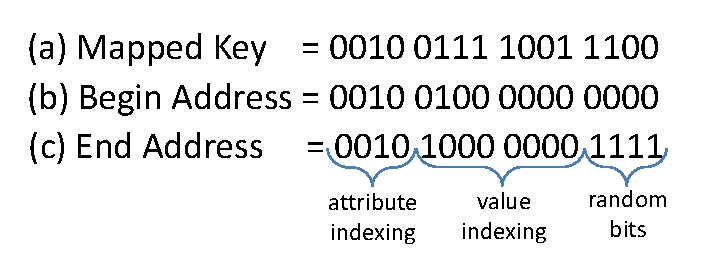
\epsfig{file=sword.eps, width=3in}
\caption{\label{fig:sword}SWORD DHT key mapping for free disk space: (a)key mapping of 121GB free disk space (b)Query begin address for 64GB free disk space (c)Query end address for 128GB free disk space}
\end{figure}
Figure~\ref{fig:sword} shows SWORD DHT key mappings. In this example, $n$ is 16 bits, $m$ is 4bits, and $k$ is 8 bits. Let us assume that value $0010$ indicates the free disk space attribute.
A node whose free disk space is 121GB sets its free disk attribute key as in Figure~\ref{fig:sword} (a).
To find nodes whose free disk space is between 64GB and 128GB, SWORD first decides the query begin address by setting attribute bits as $0010$, value bits as 64GB, and random bits as all 0x0s, shown in Figure~\ref{fig:sword} (b).
For the query end address, it sets attribute index bits as $0010$, value bits as 128GB, and random bits as all 0xFs as in Figure~\ref{fig:sword} (c).
Nodes between the begin address and end address will satisfy the query. 
Other than the above \textit{SingleQuery} method, SWORD supports the \textit{MultiQuery} method, which does not publish entire resource information to every DHT key converted from each resource attribute.
According to the their experiments, \textit{SinlgeQuery} outperforms \textit{MultiQuery}, so we analyze \textit{SingleQuery} only.
If multiple attributes need to be considered, the query range is determined based on the requirement of one randomly selected representative attribute.
To select optimal resources among multiple candidate nodes, SWORD provides an \textit{optimizer} module.
\subsection{Performance Analysis}
In this section, we compare the performance of MapReduce-based query system and SWORD analytically. 
Our analysis focuses on: (1)$N_Q$, Number of Visited Nodes to Complete a Query, (2)$L_Q$, Query Latency, (3)$B_Q$, Query Bandwidth, and (4)$B_U$, Resource Information Update Bandwidth.
We express the total number of nodes in a pool as $N$, the number of published attributes as $A_N$, the size of each attribute as $A_S$, 
and the number of attribute and value indexing bits as $I_A$, and $I_V$, respectively. In this analysis, we assume that node addresses are uniformly distributed.

\subsubsection{Number of Visited Nodes to Complete a Query}
MapReduce-based query system visits all nodes in a range to complete a query. Thus, if the entire pool is queried, $N_Q$ is $N$.
For SWORD, $N_Q$ depends on $I_A$ and $I_V$ shown in Figure~\ref{fig:sword}. As those bits increase by 1 bit, 
the query region decreases in half, so $N_Q$ is \begin{math}N/2^{(I_A+i_v)}\end{math}, where \begin{math}0\leq i_v\leq I_V\end{math}.
\begin{math}i_v\end{math} means the number of continuously identical bit from most significant bit (MSB) between query begin and end value. 
For example, if a query begin attribute value is 0x00FF and end value is 0x0FFF, \begin{math}i_v\end{math} is 4. 
\subsubsection{Query Latency}
The latency of a query depends on both $N_Q$ and query propagating method (e.g., bounded-broadcast). 
According to ~\cite{deetoo}, the latency of bounded-broadcast query dissemination follows \begin{math}O(log^2(N))\end{math}. Assuming SWORD spreads queries using bounded-broadcast,
$L_Q$ is \begin{math}O(log^2(N/2^{(I_A+i_v)}))\end{math}. The latency of MapReduce-based query is \begin{math}O(log^2(N))\end{math}.
\subsubsection{Bandwidth Usage For a Query}
Let us assume that a query message size is $S_Q$, and a response message size is $S_R$.
Using bounded-broadcast, a message is routed only to 1-hop neighbors, so bandwidth consumption for a query and response is $S_Q+S_R$.
Thus, the query bandwidth usage is \begin{math}(N_Q-1)*(S_Q+S_R)\end{math}.
$S_R$ of MapReduce-based query system does not increase linearly as Reduce results propagate through the bounded-broadcast tree, because a Reduce function summarizes results.

As we can see from the above three metrics, the query performance is closely related to $N_Q$. By using bounded-broadcast, we can complete a query
at the cost of \begin{math}O(log^2(N_Q))\end{math}, which is smaller than a flooding based broadcast cost (\begin{math}O(N_Q)\end{math}). Also, note that for large networks, a user can select $N_Q < N$, on a per-query basis, by specifying a sub-region of the entire network, trading off a reduction in the number of nodes visited with smaller query latency and bandwidth.
\subsubsection{Cost for Resource Information Update}
SWORD has to publish a node's resource information to remote nodes in order to support distributed matchmaking.
Every node has to publish its resource information, whose size is $A_N*A_S$ (neglecting serialization overhead), to $A_N$ nodes, because nodes mapped to the hashed key have to process matchmaking. 
In addition, each DHT entry has to be routed to a proper hashed key node, which takes $O(log(N))$ hops~\cite{chord}~\cite{pastry} or \begin{math}O(\frac{1}{k}log^2(N))\end{math}, where $k$ is number of short-cut connections~\cite{brunet}.
Accordingly, resource information update bandwidth consumption with update period $T$ is:
\begin{displaymath}(N*A_N*(A_N*A_S)*(\textit{Number of Hops}))/T\end{displaymath}
It shows that the bandwidth consumption is $O(A_N^2)$ and $O(N*log(N))$, which is not scalable in case of increasing number of resource attributes.
\subsubsection{Query Result Correctness}
A resource information in a DHT entry is updated with period $T$. If a query requirement is for static information (e.g., operating system), changes in value are atypical.
However, when it comes to dynamic information (e.g., current CPU load), the queried information reflects values that might be as old as period $T$. 
SWORD can make the update period $T$ shorter to keep resource information fresher, but it will result in more frequent updates and more bandwidth consumption.
In contrast, the MapReduce approach maintains dynamic information up-to-date by keeping it local to a node.
\subsection{Simulation Results}
To prove correctness of analysis and compare the performance of MapReduce-based query system and SWORD, we implemented an event-driven simulator. The simulator uses the Brunet~\cite{brunet} routing, DHT, and node management. It reuses the Brunet code base that has been extensively verified and deployed in realistic infrastructures such as PlanetLab, but it uses simulated event-driven times to allow experiments with large networks on a controlled environment.
We used the King data set~\cite{king} to set network latency between nodes and Archer~\cite{archer} in order to run simulations on a decentralized and distributed computing resources efficiently. 
We begin collecting results after one simulated hour (to let the P2P pool form and stabilize) by initiating target operations (e.g., resource query or DHT resource information update) at each node for 2-simulated hours.
For the MapReduce-based query system, each node initiates a query every 5 minutes while setting a query range as the whole network. 
In case of SWORD, we allocated 4 bits for attribute indexing, and a value field is filled with two randomly generated integer or double values to specify a desired region. 
We set a Time To Live (TTL) of SWORD's DHT entry as 30 minutes, and the entry update is performed every 15 minutes.
After running 10 simulations with different parameters, we calculate an average value.
\subsubsection{Query Latency}
Figure~\ref{fig:sim} (a) shows query latency. As we can see from the figure, the query latency grows as the number of nodes increases. To highlight relationship between query latency and a number of nodes in a pool,
we added query time ratio. The ratio is calculated as \begin{math}\frac{Query\ Complete\ Time}{Number\ of\ Nodes}\end{math} and multiplied by a constant value to make the value fit for the graph.
The ratio value decreases as the number of nodes increases, which means that the query latency is less than $O(N)$.
Though SWORD shows less query latency than MapReduce-based query system, the effect of SWORD's smaller query region is not so remarkable. 
When we set the attribute indexing size to 4 bits, SWORD query region is about 0.3\% of the entire network. 
However, the query latency decreased only about 30\% of an entire network query latency.
\begin{figure}[t]
\centering
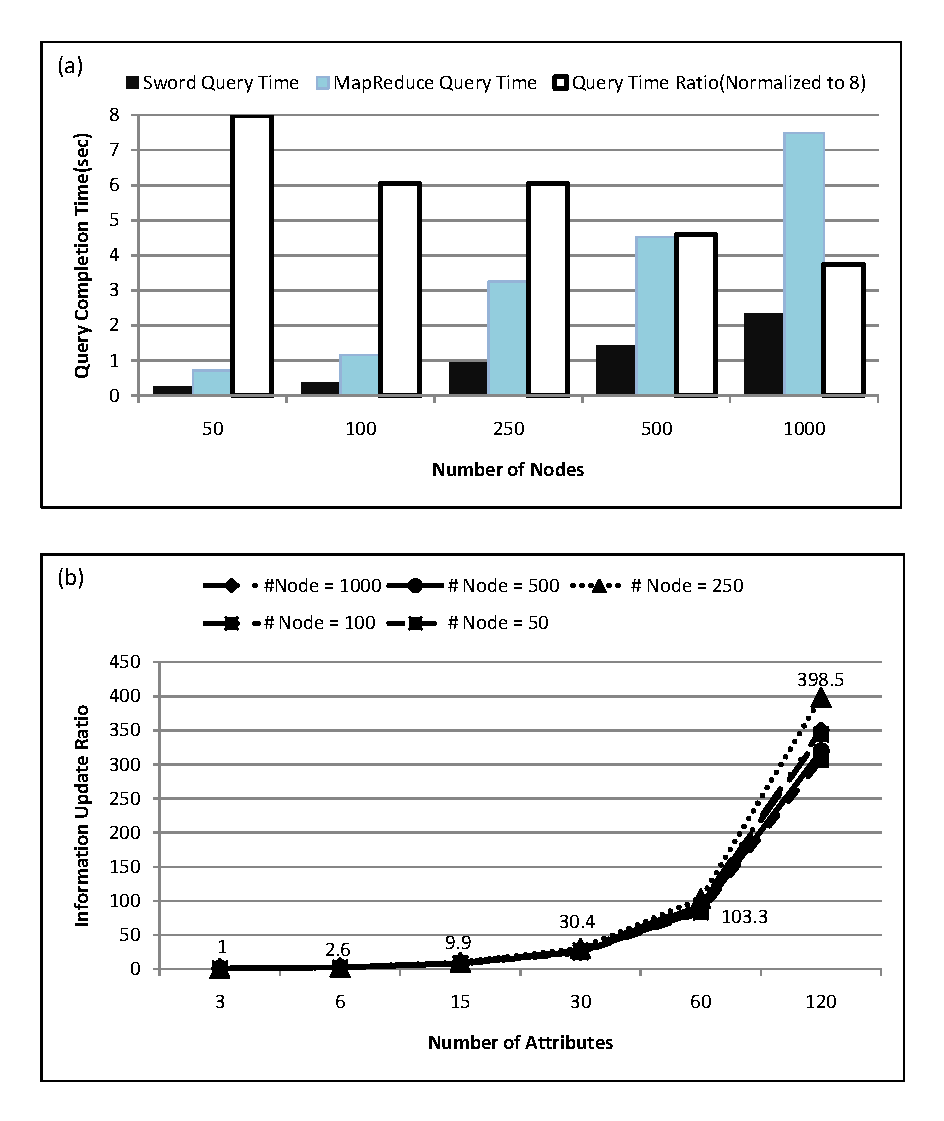
\epsfig{file=sim.eps, width=3.4in}
\caption{\label{fig:sim}MapReduce-based query system and SWORD simulation result (a) Query completion time. Query time ratio=(Query complete time / Number of nodes) * 1.6
(b) SWORD resource information update bandwidth ratio (BW consumption for $n$-attributes/BW consumption for 3-attributes)}
\end{figure}
\subsubsection{Resource Information Update Bandwidth}
Figure~\ref{fig:sim} (b) shows SWORD's resource information update bandwidth consumption\footnote{Note that the update bandwidth cost of MapReduce is zero.}  when the number of published attributes is 3, 6, 15, 30, 60, and 120. 
To show the effect of increased number of attributes, we normalized each bandwidth value to that of 3-attributes.
Thus, $n$-attribute value's ratio is calculated as \begin{math}\frac{n-attribute's\ bandwidth}{3-attribute's\ bandwidth}\end{math}. 
When the number of attributes is small, the increasing rate is not $O({A_s}^2)$, where ${A_s}$ means number of attributes, due to a resource information serialization overhead.
As the serialization overhead effect becomes negligible, the rate follows $O({A_s}^2)$. 
\subsubsection{Query Bandwidth Usage}
Table~\ref{table:bw} shows bandwidth consumption to complete a query. The \textit{Ratio} is calculated as \begin{math}\frac{SWORD Bandwidth}{MapReduce bandwidth}\end{math}. The ratio value decreases as the number of nodes
increases, but it is still bigger than 0.3\%, which is the fraction of SWORD's query region to the entire network. One possible reason is multiple hops to route a message to a node inside a query region.
The probability of finding a node in a query region decreases when the number of nodes in the pool decreases, so it will take more hops to route a message to a node in the desired region. 
In our simulation, the number of nodes inside a query region is usually zero when the number of total nodes is small. 
In case there is no node in the query region, SWORD should provide additional methods to query nodes which are located near the query region.
\begin{table}
\centering
\caption{\label{table:bw}Bandwidth Usage Per One Query}
\begin{center}
\begin{tabular}{|c|c|c|c|} \hline
\multirow{2}{*}{\# Nodes}&\multicolumn{2}{|c|}{Query BW (Bytes)}&\multirow{2}{*}{Ratio} \\ \cline{2-3}
\ &\ \ \ \ Sword\ \ \ \ &MapReduce& \\ \hline\hline
50&382&8,444&0.045\\ \hline
100&711&17,069&0.041\\ \hline
250&998&44,087&0.022\\ \hline
500&1,281&89,878&0.014\\ \hline
1000&1,841&180,428&0.01\\ \hline
\end{tabular}
\end{center}
\end{table}

Based on the analysis and simulation results, we conclude that bounded-broadcast allows propagating queries to the entire P2P network within a reasonable amount of time.
Considering that propagating a query uses less bandwidth than publishing resource information periodically, especially for large number of attributes, the MapReduce approach offers advantages over DHT-based query systems. 
In addition, propagating queries to the entire network allows each node to process matchmaking using own fresh local resource information, 
offering advantages over DHT-based query system where saved resource information might be stale.

\subsection{PlanetLab Evaluation}
The next experiment considers an actual deployment of our MapReduce system on 600 PlanetLab nodes distributed over five continents. Figure~\ref{fig:plab} shows MapReduce-based query system's query latency on PlanetLab. 
For the experiment, 3 kinds of queries were performed 100 times each. 

\textbf{Query 1}: Requirement = (Memory>1024) \&\& (KeyboardIdle > 300) \&\& (OpSys=="LINUX"). Rank = Memory + KeyboardIdle*10. Return 5 nodes whose rank is the highest.

\textbf{Query 2}: Requirement = no requirement. Rank = no rank value. Return randomly selected 200 nodes. 

\textbf{Query 3}: Requirement = (PhysicalLocation.Longitude>0) \&\& (PhysicalLocation.Latitude>0). Rank = CpuBusyTime. Return 5 nodes whose rank value is the lowest.

As we can see from the figure, 80\% of queries completed in 15 seconds regardless of the query type. However, some queries took very long to complete, 
because our query system waited for a reply from lagging response nodes until the underlying P2P system issues a RPC timeout.
This can be qualitatively explained partly by the fact that shared PlanetLab nodes are often highly loaded and by packet losses (the primary transport used is UDP).
Future work will investigate methods to handle lagging nodes other than relying on a RPC timeout of underlying P2P network.
\begin{figure}
\centering
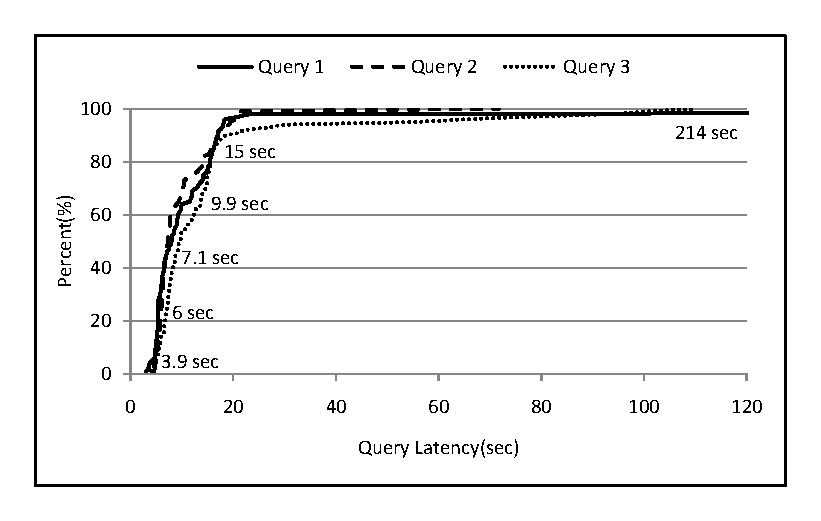
\epsfig{file=planet.eps, width=3.4in}
\caption{\label{fig:plab}Cumulative distribution of query latency on the PlanetLab with 600 nodes}
\end{figure}
\section{Related Work}
In this section, we discuss related work on P2P network range query systems and cluster monitoring systems.

\textbf{Range Query Systems on a P2P network}: Kim et. al~\cite{can_query} and Artur et. al~\cite{query_for_grid} discuss resource locating methods using a multiple dimension P2P network. 
Kim et. al~\cite{can_query} maps each resource attribute to one dimension in CAN~\cite{can}. For matchmaking, a requirement conforming zone is created based on the criteria described in a query, 
and nodes inside the requirement satisfying region are candidate ones for the query.
Artur et. al~\cite{query_for_grid} converts multiple dimension spaces into one dimension ring space. Using the correlation between multiple dimensions and an attribute value, a matchmaking is performed. 
Above methods need a local node's information update to neighboring nodes, because the information is used to select optimal requirement matching nodes.  
In addition, adding new resource attributes results in additional dimensions which bring an increased number of neighboring nodes and more management issues.\\*
Similar to our work, Kim et. al~\cite{chord_matching} and Armada~\cite{armada} use a tree-structure to check requirement matching. 
Kim et. al~\cite{chord_matching} uses Chord~\cite{chord} as an underlying P2P network. A resource information propagation tree is
constructed based on node IDs. Each node needs periodic resource information updates to the parent node, which shares same drawbacks with SWORD.
Armada~\cite{armada} assigns an Object ID based on an attribute value, and a partition tree is constructed based on the proximity of the object ID. 
To locate nodes, only the desired region of Object ID needs to be scanned. All above methods do not support arbitrary matching, such as regular expression or partial string matching.

\textbf{Cluster Monitoring System}: Blue Eyes~\cite{blueeyes} and Ganglia~\cite{ganglia} are hierarchically structured cluster monitoring systems. 
Blue Eyes~\cite{blueeyes} provides a reliable monitoring system by running multiple management servers, which are constructed as a self-organizing hierarchical tree using a management server list. 
For high system availability, monitoring data is replicated into multiple backup servers, and this replication requires much bandwidth consumption and may cause data consistency problems.
Ganglia~\cite{ganglia} uses gmond and gmetad to aggregate local resource information. 
Ganglia gmond gathers a local cluster node's information using multicast, and the gmetad accumulates inter-cluster information by collecting the gmond information.
It also consumes much network bandwidth for local node information updates to the gmond, and the system is not reliable in case of gmetad failure.
Intemon~\cite{intemon} is a server-client model monitoring system. It uses SNMP to collect resource information and supports automatic data analysis based on the historical resource correlation pattern.
Due to its static server-client relationship, it is not scalable in case multiple new clients join the monitoring system. The system also has to consume much bandwidth for periodical information update.
\section{Conclusions and Future Work}
This paper presents and evaluates MapReduce-based query system, which uses a self-organizing broadcast tree to spread queries to the entire network.
We described how our system adapted the concept of the Map and Reduce functional programming model and comparison with data processing MapReduce system.
With the aid of self-organizing bounded-broadcast trees, we can distribute queries to the entire network efficiently. 
The use of condor\_startd daemon to collect local resource information and ClassAd to process matchmaking allow us to perform various matching methods such as regular expression and  partial string matching with plentiful resource information.
Our system also supports adding new or user-defined resource attributes easily after deploying a pool without affecting performance.
The analysis and simulation results show that dispersing queries to the entire network with the bounded-broadcast method makes queries to finish in a reasonable time, 
and they also show scalability of our system for the increased number of nodes and resource attributes.
PlanetLab deployment of our system and its performance evaluation show that MapReduce-based query system is a feasible and attractable solution for a wide area resource monitoring system.
Future work in the MapReduce-based query system includes heuristics (e.g., based on machine learning) that can be applied to decrease the number of visited nodes to complete a query based on previous queries, and heuristics to allow the use of time bounds to reduce the effect of lagging nodes on query latencies.


\bibliographystyle{abbrv}
\bibliography{hpdc_mr_ws}
\balancecolumns
\end{document}